% !TeX root = ../thuthesis-example.tex

\chapter{相关工作}

\section{引言}

本章对网络流量异常检测领域的相关工作进行了综述。首先介绍了网络流量异常的定义和分类,异常检测系统的通用框架如图~\ref{fig:scheme}所示\cite{fernandes2019comprehensive}。然后介绍了流量异常领域常用的各类算法,由于本文主要工作是以循环神经网络作为基础,接下来介绍了RNN及其变体的原理,最后给出了本章小结。


% 其基础是建立一个代表正常/预期网络行为的基线轮廓,并将任何观察到的与该轮廓相比的当前活动的偏差视为异常。这个基线主要通过统计和历史网络流量数据生成。


% 异常检测是一个重要的领域,自1980年以来,国内外已经有无数学者在这方面做研究。\citet{ahmed2016survey}将异常检测技术分为分类、统计、信息理论和聚类四类。
% 待补充。



\begin{figure}
    \centering
    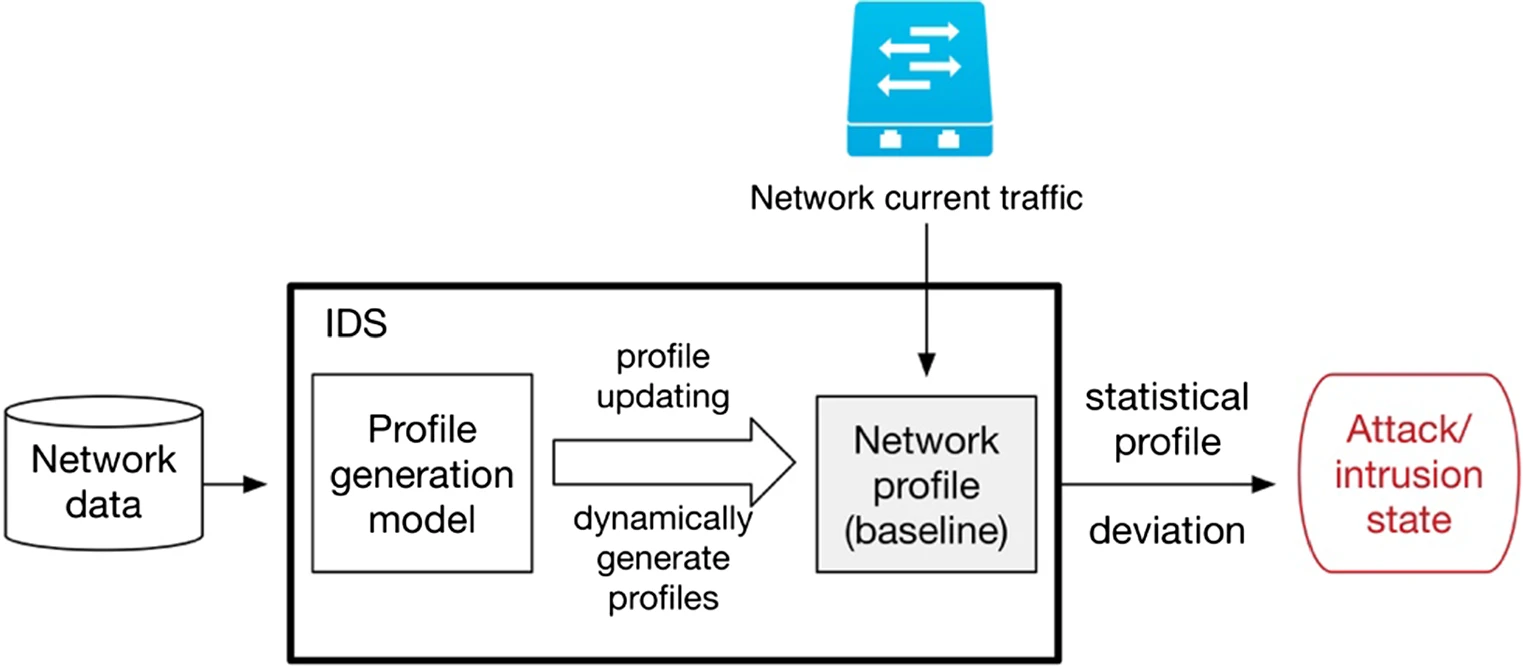
\includegraphics[width=0.6\linewidth]{异常检测技术的通用架构.png}
    \caption{异常检测的通用框架}
    \label{fig:scheme}
  \end{figure}

% 本章还讨论了用于网络入侵检测的数据集的研究挑战。



\section{网络流量异常的定义和分类}
% hawkins(1980)就此我们给出了异常的一个具有本质性的处理定义[3]:异常就是在一个随机数据集中只能表现被认为不具有所属性差异的那些随机数据,使得有人甚至可以由此怀疑这些差异数据实际上本身并非并没有任何随机的处理偏差,而是产生于一种完全不同的处理机制。
Hawkins(1980)\cite{hawkins1980identification}为“异常”下了一个定义:某些数据由于在数据集中表现出差异,因此值得怀疑这些数据不是一般的随机偏差,而是来自完全不同的机制,我们称这些数据为“异常”。例如在道路交通领域,某条道路的车流量突然增多,甚至多至堵塞,又或者突然减少,此时车流量数据就是一个异常。因此网络行为的异常就是指那些与正常的、标准的,我们所预期的行为相异的表现。为了检测网络异常,网络所有者必须有一个预期或正常行为的概念,我们称其为“基线”。要检测网络行为的异常,就需要确保基线持续稳定,如果我们在监测的过程中发现有不寻常的走向,或者有特殊事件出现,就会合理怀疑有外部的蓄意攻击导致网络流量呈现异常,以及监控指标被改变的状况。

% Hawkins(1980)给出了异常的本质性定义\cite{hawkins1980identification}:异常是在数据集中表现出差异的那些数据,使人怀疑这些数据并非随机偏差,而是产生于完全不同的机制。例如在道路交通领域,某条道路的车流量突然增多,甚至多至堵塞,又或者突然减少,此时车流量数据就是一个异常。因此网络行为的异常就是指那些与正常的、标准的,我们所预期的行为相异的表现。为了检测网络异常,网络所有者必须有一个预期或正常行为的概念,我们称其为基线。要检测网络行为的异常,就需要持续监控网络中的意外趋势或事件,那些可能改变网络流量特征或者监控指标的恶意行为。


本文只关注引起网络流量特征变化的恶意行为,而对于系统权限提升,缓冲区溢出等黑客攻击手段暂时不做研究。


网络流量异常具体有哪些类别,学术界没有统一的意见。本文中关注的网络流量异常按照产生意图分为恶意和非恶意两类,其中恶意行为主要有拒绝服务攻击、网络扫描、BGP劫持、网络蠕虫、僵尸网络等;非恶意行为主要有物理故障、突发事件等。接下来我们对这些异常分别进行介绍:

\begin{itemize}
  \item 拒绝服务攻击(Denial of Service,DoS):攻击者往往通过构造大量请求访问目标主机,使其无法处理正常的流量请求,导致正常用户被拒绝服务。
  \item 网络扫描:攻击者在发动网络攻击之前,普遍会先进行网络扫描,否则,黑客可能会向未启动的主机发送恶意报文,从而增加攻击的成本。所以他们总是要先在某个子网范围内扫描出活跃的主机以及可访问的端口。为了以最低代价寻找到可攻击的目标,网络扫描通常是网络攻击的前奏。
  \item BGP劫持:BGP劫持是指通过一个自治系统错误宣称IP为其所有,使得使用边界网关协议维护的互联网路由表的路由器错误地将用户发送的数据传送给非数据传送目的地。
  \item 网络蠕虫:网络蠕虫通过网络和电子邮件进行复制和传播,它们首先搜索并且识别出本身具有缺陷的通信端点,在对这些端点施加攻击后,又经由局部地区的私有网路或者庞大的互联网扩散到其他通信端点。例如“熊猫烧香”及其变种就是蠕虫病毒。
  \item 僵尸网络:僵尸网络指由感染了恶意软件的计算机组成的网络,这些计算机集群由攻击者控制。
  \item 物理故障:物理故障也就是指现实世界中的设备有了损坏,包括但不限于电源与设备未连通、路由器无法传输讯息、链路间无法连接、线缆破损等意外事故。
  \item  突发事件:突发事件是指引起网络瞬时拥塞的事件,有可能是管理员配置错误,也有可能是正常的网络操作,如某网站访问量激增。
\end{itemize}

\section{网络流量异常检测算法}


本节将介绍在异常检测领域主流的一些算法,根据所依赖的技术原理的不同,将这些算法分为了基于分类、基于统计、基于聚类、基于信息论的异常检测算法。

\subsection{基于分类的异常检测算法}

% 基于分类的技术依赖于专家对网络攻击特征的广泛了解。当网络专家向检测系统提供详细的特征时,具有已知模式的攻击一经发起就能被检测出来。这完全依赖于攻击的签名,作为一个系统,只有当网络专家较早地提供了攻击的签名,它才能够检测出攻击。这说明一个只能够检测到它所知道的系统很容易受到新的攻击,而新的攻击会不断出现不同的版本,并且更加隐蔽地发起。即使创建了新的攻击的签名并将其纳入系统中,最初的损失也是不可替代的,而且修复程序非常昂贵。


% 基于分类的方法依赖于建立知识库的正常流量活动特征,并将偏离基线特征的活动视为异常活动。这种方法的优势在于它们能够检测到完全新颖的攻击,
% 假设这些攻击表现出大量的偏离正常基线的情况。需要注意的是,由于知识库中未包含的正常流量被认为是攻击,因此会产生无意中的误报。为了避免这种情况,异常检测技术需要进行训练,以建立正常的活动基线,这个建立基线的过程通常非常耗时,而且还取决于是否有完全正常的流量数据集。在实践中,获得无攻击的流量实例是非常罕见且昂贵的。此外,在如今信息更新变换快速的动态网络环境中,保持正常基线的更新是非常困难的。
本文在现有的大量基于分类的网络异常检测技术中,主要讨论以下三种技术,“支持向量机”(Support Vector Machine,SVM),“贝叶斯”(Bayes)以及“神经网络”(Neural Network, NN)。

\subsubsection{支持向量机}
Eskin等人\cite{2002AEskin} 引入无监督SVM的概念来检测异常事件。常规的SVM的原理是推导出一个超平面,使得正类样本和负类样本之间的分离余量最大化,将特征空间中的两类数据进行分离。标准的SVM算法是一种监督学习方法,需要标记数据来创建分类规则。而该算法经过改进SVM,试图将整个训练数据集从原点分离出来,找到一个以最大余量将数据实例与原点分离的超平面。

Hu等人\cite{Hu2003Robust} 提出了一种忽略噪声数据的异常检测方法,该方法使用Robust SVM(RSVM)来开发。标准的SVM有一个主要假设,即:“所有的训练样本数据都是独立且相同分布的(i.i.d)”。但是在实际场景中,训练数据往往包含噪声,这就会导致标准SVM会学习出一个高度非线性的决策边界,从而导致通用性较差。有鉴于此,RSVM以类中心的形式加入了平均化技术,使得决策面更加平滑。此外,RSVM另一个优点是能大大降低支持向量的数量,从而减少运行时间,提高效率。

% Taeshik Shon等人\cite{shon2005machine} 提出了一种基于增强支持向量机(Enhanced Support Vector Machines)的异常检测算法。增强支持向量机是该文作者提出的一种新型的支持向量机,该向量机同时具备了传统支持向量机的高性能和单类支持向量机检测新异常的能力。在预处理阶段,检测算法使用数据包过滤器滤除畸形数据包。随后,检测算法使用遗传算法对数据包头的信息进行特征选择。接下来,检测算法利用SOM网络对正常流量进行聚类,并用这些聚类来训练增强支持向量机,从而得到最终的异常检测器。

% Taeshik Shon 等人\cite{shon2005machine}设计了一种此前未有的增强支持向量机(Enhanced Support Vector Machines),这种支持向量机的工作能力结合了以往传统支持向量机与单类支持向量机二者已有的优点,不仅性能优良而且也能较好的识别出新出现的异常。增强支持向量机的训练过程也需要经过预处理的几个步骤,首先是用数据包过滤器排查且删除异常数据包。接着是对数据包头进行处理,这个阶段利用到的是“遗传算法”,会从原始存在的所有特征进行属性选择。在剔除多余无用的特征,且使用自组织映射网络针对正常流量实行聚类之后,会生成样本集合。用这些样本集合训练最新的支持向量机,我们所需的异常检测器就产生出来了。


\subsubsection{朴素贝叶斯}

朴素贝叶斯是一个简单的概率分类器,通常用于网络入侵检测问题。 它将先验信息与样本信息结合起来,并以统计推论的方式进行实施,从而利用概率显示出各种形式的不确定性。 朴素贝叶斯假设了所有输入属性在条件上都是彼此独立的。

Kruegel等人\cite{kruegel2003bayesian} 假设异常检测系统包含许多模型,用于分析一个事件的不同特征。他们指出了在这种系统下异常检测技术造成高误报率的两个主要原因:一是异常检测系统通过将多个概率模型的输出进行汇总,而每个模型往往只给出一个事件的常态/异常的得分或概率,从而导致高误报率;二是异常检测系统无法处理那些不正常但合法的行为,如CPU利用率、内存使用率突然增高等。基于贝叶斯网络的概念,Kruegel\citep{kruegel2003bayesian}指出可以使用一种方法降低误报率,该方法能够正确处理那些在合法范围内稍显不正常的行为。对于一个输入事件的有序流($\symbf{S}=e_1,e_2,e_3...$),异常检测系统决策每个事件是正常还是异常。该决策基于k个模型($\symbf{M}=m_1,m_2,...,m_k$)的输出($o_i|i=1,2,...,k$)和可能的附加信息($\symbf{I}$)。应用贝叶斯网络来识别异常事件,引入根节点,根节点代表一个具有两种状态的变量。一个子节点用于捕捉模型的输出,子节点与根节点相连,预计当输入异常或正常时,输出事件会有所不同。

\subsubsection{神经网络}

神经网络是深度学习的热门技术,早已在多个方面实践成功,但其对计算量的要求很高。神经网络对数据进行分类的优势也可被用于网络异常检测。在网络异常检测领域,神经网络通常会和其他技术进行结合,如统计方法。


Hawkins等人\cite{hawk2002Outlier}提出了一个多层的前馈神经网络,该神经网络可以用来进行异常值的检测。这个多层前馈的神经网络(multi-layer feed-forward neural networks)也就是Replicator Neural Networks。具体而言,它的运行方式是设置了三个隐藏层,夹在输入层和输出层的中间,目标是通过训练,使输出层能以最小的误差重现出输入的数据模式。其原理在于输入层与输出层节点的数量比隐藏层节点的数量要多,因此隐藏层能够具有压缩数据和恢复数据的作用。Replicator Neural Networks的示意图如图~\ref{fig:rnn}所示。

% Hawkins等人\cite{hawk2002Outlier} 提出了一个多层的前馈神经网络,该神经网络可以用来进行异常值的检测。具体来说,Replicator Neural Networks是一个多层前馈的神经网络 (multi-layer feed-forward neural networks),在输入层和输出层之间放置了三个隐藏层,它的目标是通过训练在输出层以最小的误差重现出输入的数据模式。由于该模型中间隐藏层节点的个数少于输入输出层节点的个数,这样就起到了压缩数据和恢复数据的作用。
% Replicator Neural Networks的示意图如图~\ref{fig:rnn}所示。

\begin{figure}
    \centering
    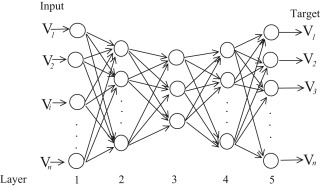
\includegraphics[width=0.6\linewidth]{RNN.jpg}
    \caption{Replicator Neural Networks示意图}
    \label{fig:rnn}
  \end{figure}

  \citet{2001HIDE} 提出了一种分层入侵检测模式,这是他在神经网络的技术基础上搭配了统计方法建立的模型,此系统用一个连续变量($t$)表示神经网络分类器的输出,若变量为1那么当前没有攻击,而-1出现时则是确切的入侵。
  
  除了统计模型,自组织映射(Self-Organizing Map,SOM)亦被用于网络异常检测。Ramadas等人\cite{2003Detecting}提出,由于SOM基于一个假设:即网络攻击可以由不同的神经元组来描述,这些神经元组与其他神经元组相比,在输出神经元图上覆盖更大的区域。因此利用SOM,可以对网络流量进行实时分类。
  
  Poojitha等人\cite{Poojitha2010} 设计出了一种前馈神经网络,使用的训练算法是“反向传播算法”,该模型的要点在于学习出系统无异常期间所表现出的活动模式,并且将违反此期间的行为归类于异常。

\subsection{基于统计的异常检测算法}
从前检测异常是使用假设-检验的方法,也就是要利用统计与概率模型。第一步是预测数据的分布,并从中找到预先认定的“异常”,在此操作下总是使用极值分析或假设检验。也就是说,当前存在基础的一维数据时,首先拟定数据是遵守正态分布的,若有超出均值达到某个范围外的点,就认定是异常点。此操作推广到高维后,假设各个维度相互独立。这类方法的好处是速度比较快,但是因为总要进行“假设”,所以效果不一定很好。因此统计技术的主要挑战是减少固定阈值引起的误报\cite{cormode2010algorithms}。例如,可以使用统计信号处理程序来提高检测率,同时减少误报,如Lakhina等人在主成分分析工作中所做的工作\cite{lakhina2004diagnosing,lakhina2004structural,lakhina2005mining}。

% 早期的异常检测方法往往基于统计与概率模型,也就是假设-检验的方法。首先对数据的分布做出假设,然后找出假设下所定义的“异常”,因此往往使用极值分析或假设检验。比如对最简单的一维数据假设服从正态分布,然后将距离均值某个范围以外的点当做异常点。推广到高维后,假设各个维度相互独立。这类方法的好处速度一般比较快,但是因为存在很强的“假设”,效果不一定很好。因此统计技术的主要挑战是找到减少硬阈值引起的误报产生的方法\cite{cormode2010algorithms}。例如,可以使用统计信号处理程序来提高检测率,同时减少误报,如Lakhina等人在主成分分析工作中所做的工作\cite{lakhina2004diagnosing,lakhina2004structural,lakhina2005mining}。

Nong等人\cite{Nong2010An}基于卡方检验的距离测量方法,将卡方检验的理论应用于异常检测。根据此技术,首先需要建立一个正常事件的基线,然后将偏离统计值的点视为异常。基于chi-square检验统计量的距离测量方法为:
\begin{equation}
    \chi^2 = \sum_{i=1}^n \frac{(X_i - E_i)^2}{E_i}
\end{equation}
其中$X_i$表示的是第$i$个变量的观测值,$E_i$表示的是第$i$个变量的期望值,变量的数量以$n$表示。当一个变量的观测值接近预期时,$\chi^2$的值就会很低。根据$3\sigma$定律,当观测值的$\chi^2$大于$\bar{X^2}+3S_X^2$时,该值被视为异常。

\subsubsection{小波分析} 
小波变换的基本原理涵盖在傅里叶变换的过程当中,起初三角函数基是无限长的,通过小波变换将其变成长度有限且会衰减的小波基。强大的基函数小波,在时间和频率上是局部的,允许被表示的序列和它们的系数之间有密切的联系。如此一来频率得以获取,同时还可以定位到时间。
% 小波分析的重点是对非稳定数据序列进行建模,这种数据序列可能包含在长时间内振幅和频率都会变化的信号。小波变换的基本原理是在傅里叶变换的过程中,将基由无限长的三角函数基换成有限长的会衰减的小波基。小波是强大的基函数,在时间和频率上是局部的,允许被表示的序列和它们的系数之间有密切的联系。这样不仅能够获取频率,还可以定位到时间。


Callegari等人\cite{callegari2011combining}提出了一种利用小波与基线相结合的实时异常检测方法。它是通过提取NetFlow轨迹,并将其转化为ASCII数据文件,进行路由器级别的分析。经过格式化后,通过哈希函数将不同的流量汇总到基线中。然后,将时间序列数据进行小波变换,若发现不连续点则视为异常点。

另一项使用小波的研究是由Hamdi等人\cite{hamdi2007detecting}产生的。它依赖于通过区分危险和非威胁性的异常来识别与攻击相关的异常。这项任务是在周期观测概念的基础上完成的,小波理论被用来分解一维信号,以分析其特殊频率和时间定位。

\subsubsection{主成分分析}
通常情况下,“主成分分析”(Principal component analysis,PCA)方法的用法是将原本在高维空间里面的数据点,以投影法降至低维空间内。但是我们也可以将之用于检测网络流量异常这个领域。该方法的主要原理是将特征空间为$n$的原数据集映射到新的更小的特征空间$k$中,新特征即为主成分(PC),其中$k<<n$,这些 PC是一组正交向量,它们构成了一个$k$维子空间。同理,异常点的判别方法,是将存在于初始空间内的那些数据, 映射到主成分空间,接着再把投影拉回到原始的空间。假如进行投影和重构的数据只包含第一主成分,那么大多数的数据在重构前后误差值不大;但是对于异常点而言,重构之后的误差,相较此前的误差值依然很大。

% 主成分分析(Principal component analysis, PCA)是一种常见的降维方法,也可以用于网络流量异常检测领域。该方法的主要原理是将特征空间为$n$的原数据集映射到新的更小的特征空间$k$中,新特征即为主成分(PC),其中$k<<n$,这些PC是一组正交向量,它们构成了一个$k$维子空间。为了发现异常点,基于主成分分析(PCA)的算法会把原始数据从原始的空间投影到主成分空间,然后再把投影拉回到原始的空间。如果只使用第一主成分来进行投影和重构,对于大多数的数据而言,重构之后的误差是小的;但是对于异常点而言,重构之后的误差依然相对大。

Lakhina等人\cite{lakhina2004diagnosing} 利用主成分分析法对流量测量结果进行二分,分为正常和异常两类。主成分分析是基于将一组网络流量测量所占的高维空间分离成不相干的子空间,分别对应正常和异常的网络条件。PCA 的结果是$k$个子空间,对应正常的网络流量行为,至于剩下的$m$个子空间($m=n-k$) 的组成成分则是异常或噪声。接下来需要通过制定有差异的阈值,使这些结果中的异常流量被检测出来。这时的做法是将每一个新的流量测量值一一投射到$k$和$m$这两个子空间上。

% 利用主成分分析法将测量结果区分为正常和异常两个子空间,能有效地处理流量异常的判定困难。这个方法是基于将一组网络流量测量所占的高维空间分离成不相干的子空间,两个子空间分别对应正常和异常的网络条件。使用主成分分析法得到的是$k$个子空间,这是与符合一般规律的网络流量行为相应的;至于剩余的$m$ 个子空间($m=n-k$),则是与异常和噪声对应。接着再把每一个新的流量测量值投射到这$k$和$m$两种子空间上。这样就可以通过区别开相异的阈值,使得测量出的异常值被从正常测量值中划分开来。

% 利用PCA将流量测量结果有效地分离为正常和异常子空间,解决了网络流量的异常诊断问题。该方法是基于将一组网络流量测量所占的高维空间分离成不相干的子空间,分别对应正常和异常的网络条件。PCA的结果是$k$个子空间,对应正常的网络流量行为,而剩余的$m$个子空间($m=n-k$)则由异常和噪声组成。然后,将每一个新的流量测量值映射到这两个子空间上,这样就可以通过设置不同的阈值将这些测量值划分为正常或异常。

Pascoal等人\cite{pascoal2012robust}提出的异常检测方法采用了鲁棒PCA检测器与鲁棒特征选择算法合并,以获得对不同网络背景和环境的适应性。该鲁棒PCA与经典的PCA方法相反,它对异常值不敏感,并且无需使用可靠标记的数据集进行训练。

Fernandes等人\cite{fernandes2016network}发表了根据统计程序主成分分析生成出的一种异常检测算法。这种算法首先生成一个“使用流量分析的网络段数字签名(DSNSF)”的网络基线,然后将该基线与真实网络流量进行比较以识别异常事件。该系统分析了几天内的历史网络流量数据,从中找出最重要的流量时间间隔,同时对数据集进行了缩减,使新的缩减集能够有效地描述正常的网络行为。然后,以DSNSF作为阈值,通过得到的PCA参数,限制一个区间,偏离阈值的被认为是异常的。该系统共使用七个流量特征,三个IP流量特征(bits/s, packets/s, flows/s)被用来生成DSNSF,四个流量属性(源IP地址、目的IP地址、源TCP/UDP端口和目的TCP/UDP端口)被用来生成一个包含有关异常流量间隔的信息报告。这种方法的缺点是只针对流量属性进行判定异常,只考虑检测基于流量的攻击。


\subsubsection{协方差矩阵}

协方差矩阵是二阶统计,已经被证明是一种强大的异常检测方法。该领域的一个有趣的方向是寻找哪些变量最能标记网络异常,用以提高检测性能。

Yeung等人\cite{yeung2007covariance}采用协方差矩阵分析来检测洪泛攻击。该方法将网络流量建模为协方差矩阵样本,以利用时序样本中包含的统计量达到检测泛洪攻击的目的,直接利用协方差矩阵的变化和相关特征的差异来揭示正常流量与各种类型的洪泛攻击之间的变化。


 Miao Xie等人\cite{xie2014segment}研究了一种基于段的方式处理数据的技术。因为在无线传感器网络(WSNs)中,人们观察到大多数异常事件都会持续相当长的时间。由于现有的异常检测技术通常是以基于点的方式单独处理每个观测值,它们无法可靠和有效地报告在单个传感器节点中出现的这种长期异常。因此该方法采用斯皮尔曼等级相关系数(Spearman's rank correlation coefficient 或 Spearman's $\rho$)和差分压缩概念近似的样本协方差矩阵,以大幅降低计算和通信成本。







% \citet{Christopher2002Service} 提出了一种用于检测异常网络流量的统计处理单元,更具体地说,是为了检测R2L和U2R等罕见的攻击。开发了一种度量方法,使系统能够自动搜索不同服务请求的相同特征。根据以下三个主要特征计算出请求的异常得分。
% 请求的类型;
% 请求的长度;以及
% 有效载荷分布。
% 网络管理员定义了一个阈值,以便对异常请求发出警报。异常得分的计算方法如式(5),其中有效负载分布的权重大于其他属性。(5)
% 基于统计学理论的原理,我们开发了不同类型的技术来检测异常,接下来将讨论。

% 在时间序列异常检测领域,最常见的基于统计的算法为ARIMA,即差分自回归移动平均模型[8]。我们将流量信号分解为两部分,一是遵循一定规律、可预测的正常变化,二是由突发性变化组成、不可预测的异常情况。ARIMA分析和建模用于网络流量预测,能够检测和识别流量异常或异常值。


\subsection{基于信息论的异常检测算法}

信息论是一门以信息量化和冗余分析为核心的数学学科,其前身是1948年Claude E. Shannon在寻求信号处理和通信操作的数据压缩、传输和存储时提出的设想\cite{shannon1948mathematical}。然而,它的应用扩展到许多其他领域,如电子通信、决策支持系统、模式识别等。常用的信息理论测量方法有香农熵、广义熵、条件熵、相对熵、信息增益和信息成本等。信息论应用于异常检测的途径主要是依靠计算流量特征的相互信息或熵值来识别异常分布。

\subsubsection{熵}
% 熵(entropy)是接收的每条消息中包含的信息的平均量,可以理解为不确定性的度量,因为越随机的信源的熵越大。
熵(entropy)在实验中可以当作是不确定性的度量, 因为它是根据收到的每条消息中所包含的信息,平均后得出的量值,所以信息来源越随机,熵的值就越大。
异常检测领域中,熵可以有效地将流量特征描述为分布,例如源/目的端口或IP地址,因为有某些类型的异常会对严重影响这些分布。通过这种方式,可以检测到例如由目的端口熵的变化表示的端口扫描攻击。

Behal等人\cite{behal2017detection}指出,由于DDoS攻击和突发事件会引起网络流量模式的大幅改变,而基于信息理论的熵或散度可以快速捕捉网络流量行为中的这种差异。因此,他们提出了一种利用流量之间的熵差进行异常检测的算法。通过采用了一组泛化的$\phi$-熵和$\phi$-散度,检测合法流量和攻击流量之间的信息距离。经过实验,该算法对于突发事件和DDoS的检测精度较高,而在其他数据集上表现一般。

David等人\cite{david2015ddos} 提出了一种通过快速熵和基于流量的分析来增强对DDoS攻击的检测的方法。作者将观察到的流量汇总成一个单一的流量,并考虑到每个连接在一定时间间隔内的流量数,而不是取每个连接的数据包数。第二步基本上是计算每个连接的流量计数的快速熵。最后,根据快速熵和流量计数的均值和标准差生成一个自适应阈值。阈值随流量模式状况不断更新,提高了检测精度,同时快速熵的使用减少了计算处理时间。

% Amaral等人[129] 提出了一种基于流量特征的异常检测系统,该系统同时使用IP Flow属性和图表示。该算法基于香农熵的一种泛化类型,Tasallis熵。和香农熵的主要区别在于它有一个参数可以定义 对熵的结果有贡献。通过调整异常检测器的敏感性,使其能够适应不同类型的网络,并检测出更多类型的攻击。

% Bhuyan等人[130]提出的工作带来了一种基于离群值的异常检测方法,使用广义熵和互信息来创建一种能够选择相关的、非冗余的特征子集的特征选择技术。作者认为,由于相互信息降低了一个随机变量的不确定性,而广义熵衡量了数据中的不确定性量,因此他们使检测速度更快,更准确。

% 此外,Berezinski等人[131]为了检测现代僵尸网络恶意软件,引入了一种基于香农熵的网络异常检测器。他们的方法创建了一个网络配置文件,它存储了5分钟滑动时间窗口中的最小和最大熵值。这些值被用于与观察到的熵进行比较。这定义了一个阈值,因此,可以识别不同特征分布的异常分散或集中。最后,作者使用流行的分类器,如决策树和贝叶斯网络,以便对异常进行分类。



\subsubsection{KL散度}
KL散度,又称相对熵,通常用于测量一个随机变量$X$的真实概率分布$P$与任意概率分布$Q$($P$的近似)之间的差异。设 $p(x)$、$q(x)$是离散随机变量 $X$ 中取值的两个概率分布,则 $p$ 对 $q$ 的相对熵是:
\begin{equation}
    D_{KL}(p||q) = \sum_x p(x) \log \frac{p(x)}{q(x)} = E_{p(x)} \log \frac{p(x)}{q(x)}
\end{equation}
在机器学习中,$P$往往用来表示样本的真实分布,$Q$用来表示模型所预测的分布。


Xie等人\cite{xie2016distributed} 利用KL散度着重检测了无线传感器网络(WSN)中的一种特殊类型的异常,这种异常会同时出现在邻近节点的集合中,并持续相当长的时间。基于节点的技术在此场景下效果和效率都不尽如人意。作者提出了基于分布式段的递归核密度估计,通过计算两个时间段的概率密度函数的差异,来判断是否发生了异常。同时也为了以较低的通信成本实现分布式估计,作者采用KL散度作为度量方法。利用真实世界的数据集对算法进行评估,结果表明,该算法可以以更低的通信成本实现很好的性能。

Li等人\cite{li2012differential} 以检测无线传感器网络中的异常数据值为目标,提出了一种基于差分KL散度的异常检测方案。该方案首先将整个传感器网络划分为若干个簇,每个簇中的传感器在物理上相互接近,并且具有相似的感知值。然后,在每个簇内使用KL散度,以通过统计测量两个数据集之间的差异来检测异常值。他们的工作取得了良好的检测率和较低的误报率,同时比其他文献中的类似研究消耗更少的CPU、内存等资源。



% Ambusaidi等人(2014)中提出了一种基于非线性相关系数(NCC)的相似性测量方法,以提取网络流量之间的线性和非线性相关性。提取的相关信息用于检测恶意网络行为。Pearson׳s相关系数是一种基本的线性相关方法,用于找出两个变量之间的依赖关系(Ahmed等,2015c),然而,在一些数据集中,不同变量之间存在非线性相关,如网络流量中。NCC由Wang等(2005)定义,如式(18),其中和为变量X和Y的修正熵。

% 给定一组m个正常训练数据实例,首先计算NCC。对于任何传入实例,传入实例与正常实例之间的NCC记录为 。对于用户定义的阈值σ,其范围在0和1之间,如果NCC的差异大于σ,则认为一个传入流量实例是异常的(19)。


% 在Tan等(2014a)中,针对DoS攻击检测,提出了一个利用多元相关分析(MCA)的系统,通过提取网络流量特征之间的几何相关性,来实现网络流量的精确特征分析。检测过程主要包含三个步骤,如图6所示。在步骤1中,在一个明确的时间区间内生成基本特征。第2步包含多元相关分析,应用 "三角区域图生成 "模块,提取第一步得出的每个流量实例中两个不同特征之间的相关性。第三步是基于训练和测试阶段的决策。


% 基于这些知识,可以建立适当的异常检测模型。有监督的异常检测技术需要先有一个训练数据集,再有一个测试数据来评估模型的性能。在这种情况下,首先,使用信息理论措施来确定模型是否适合测试新数据集。Noble和Cook(2003)在基准DARPA和UNM审计数据集上进行了实验,以证明信息理论措施的效用,并得出结论,它们可以用来创建高效的异常检测模型,也可以用来解释它们的性能

% Tan等人(2014a)中的多变量相关分析方法的概念被纳入到网络流量实例的表征中,并将其转换为相应的图像。这些图像被用于DoS攻击检测,基于一个广泛使用的异构度量,即地球移动者距离(Earth Mover׳s Distance,EMD)(Rubner等,1998)。EMD考虑了跨区域匹配,比其他一些著名的异同度测量方法更准确地评估了分布之间的异同度。

\subsection{基于聚类的异常检测算法}

% 聚类分析是把彼此相似的对象分成不同的组别,组内的对象是相似的(相关的),而不同组之间是不同的(不相关的)。如果组内的相似性越大,组间的差别越大,说明聚类的效果越好。因此,聚类技术可以用于离群值检测(Outlier Detection),识别出与正常组别相距较“远”的值,判定为异常值/离群值\cite{2012Cluster}。聚类算法通常是基于距离/密度发现异常点。其关键步骤在于给每个数据点都分配一个离散度,针对给定的数据集,对其中的任意一个数据点,如果在其局部邻域内的点都很密集,那么认为此数据点为正常数据点,而异常点则是距离正常数据点最近邻的点都比较远的数据点。通常由阈值进行距离远近的界定。


Rajasegar等人\cite{2014Hyperspherical}发明了一种聚类算法,是根据分布式超球面集群得出的,主要作用在于检查测试无线传感器网络中有无异常。
检测过程是以聚类法进行建模,对象是每个端点的流量数据。建模后还要使用k 个最近邻(KNN)集群的平均集群之间的距离去辨认出异常集群,辨认后就可以将数据向量分类为正常或异常。该算法的特点是操作过程在分布式系统中,通过传感器端点指出集群聚类的信息。在与其他端点传递信息之前,先凭借中间节点的先行合并,能使得通信开销降至最低。
% 提出了一种基于分布式超球面集群的聚类算法,用于检测无线传感器网络中的异常。
% 该算法利用聚类对每个节点的流量数据进行建模,通过使用k个最近邻(KNN)集群的平均集群间距来识别异常集群,就可以将数据向量分类为正常或异常。该算法的特点是在分布式系统下进行,传感器节点上报集群聚类的信息,在与其他节点通信之前,由中间节点先行合并,从而使得通信开销最小化。


K-means 虽然有局部收敛性和在簇中心节点选择上具有敏感性这些缺点。但是它仍然是一种经典的聚类技术,能够将数据划分为不同的类别。由于这种技术十分热门,有相当多的技术人员尝试着想借助其他技术来优化k-means,去改善k-means的不足之处。Karami等人\cite{2015Karami} 就设计了一种基于“粒子群优化”(particle swarm optimization,PSO) 和k-means 与局部优化混合的模糊异常检测系统,以确定最优的簇数。



Carvalho等人\cite{carvalho2016unsupervised} 开发了一种主动式网络监控系统,可以检测异常事件,减少决策中的人工干预和错误概率。他们提出一种创建网络基线轮廓DSNSF(使用流量分析的网段数字签名)的方法。该方法通过修改蚁群优化算法,使用聚类方法描述正常的网络使用情况,该方法称为ACODS。ACODS在大量高维输入数据中,通过无监督学习机制优化提取行为模式,对网络流量发现进行表征。然后为了检测异常行为,他们首先计算每个时间区间内真实流量与正常曲线的相似度;然后计算序列之间的距离,并提供基于距离的测量方法。
作者所提出的告警系统采用七种流量属性(Bits, Bytes, Flows, Origin IP, Destination IP, Origin Port, Destination Port)工作,利用熵来计算IP地址和端口特征的相关信息。当检测到异常时,ACODS会提供一份包含IP流量信息的完整报告,说明每个属性对检测到的异常时间间隔的影响。ACODS具有平方复杂度,导致解的收敛要经过多次迭代,作者试图通过使用局部搜索和信息素更新来缓解。

Dromard等人\cite{dromard2016online} 所设计的无监督异常检测器,是建立在网格增量聚类算法和离散时间滑动窗口之上的。网格增量聚类在众多聚类算法当中效率拔群,因为后者只更新之前的特征空间分区,而不是每当增加或删除很少的点时,就对整个空间进行重新分区。也因此,网格增量聚类的使用是在帮系统减少繁复性,并且使其在实时检测方面效能更强。最后系统合并这些更新的分区,用以识别最不相似的异常值。

% 提出了一种基于网格增量聚类算法和离散时间滑动窗口的无监督异常检测器。网格增量聚类比常规的聚类算法更有效率,因为后者只更新之前的特征空间分区,而此前的做法是每当对点的数目进行增删时,哪怕更改的点不多,也会对整个空间做重新分区的处理。增量网格聚类的使用有助于降低系统复杂度,从而使其在实时检测方面更加可行。最后系统合并这些更新的分区,用以识别最不相似的异常值。


Syarif等人\cite{2012syarif} 在NSL-KDD数据集上系统对比了各种聚类算法的性能,他们选出了5种应用最广泛的聚类算法:k-means、改进的k-means、k-medoids、EM算法和基于距离的异常检测算法。实验表明,在同等水平的误报率情况(约21\%)下,基于距离的异常检测算法效果最好,准确率为80.15\%,k-means算法效果最差,准确率为57.81\%。
% 表\ref{聚类算法}展示了这些算法在NSL-KDD数据集下的性能表现。

% \begin{table}[]
%   \caption{聚类算法在NSL-KDD数据集的性能对比}
%   \label{聚类算法}
%     \centering
%     \begin{tabular}{@{}clllclcl@{}}
%     \toprule
%     \multicolumn{4}{c}{Algorithm}                          & \multicolumn{2}{c}{Accuracy(\%)} & \multicolumn{2}{c}{False positive(\%)} \\ \midrule
%     \multicolumn{4}{c}{k-means}                            & \multicolumn{2}{c}{57.81}        & \multicolumn{2}{c}{22.95}              \\
%     \multicolumn{4}{c}{Improved k-means}                   & \multicolumn{2}{c}{65.4}         & \multicolumn{2}{c}{21.52}              \\
%     \multicolumn{4}{c}{k-medoids}                          & \multicolumn{2}{c}{76.71}        & \multicolumn{2}{c}{21.83}              \\
%     \multicolumn{4}{c}{EM clustering}                      & \multicolumn{2}{c}{78.06}        & \multicolumn{2}{c}{20.74}              \\
%     \multicolumn{4}{c}{Distance-based   anomaly detection} & \multicolumn{2}{c}{80.15}        & \multicolumn{2}{c}{21.14}              \\ \bottomrule
%     \end{tabular}
%     \end{table}
% 异常检测方法的一些主要局限性基本上是:没有标签数据;发现新的未知异常模式;噪声数据;高误报率。为了克服这些问题,Bigdeli等人[103]提出了一种基于增量两层集群的异常检测结构。其核心思想是对网络数据进行聚类,并将这些聚类表示为高斯混合物模型,因此该模型可以对新的实例进行分类,也可以检测并忽略冗余的实例。此外,针对误报率较高的问题,采用集体标记的方法,对新入库实例进行集体标记和增量标记。


% 聚类指的是无监督学习算法,它不需要预先标记数据来提取相似数据实例的分组规则(Jain等,1999)。虽然有不同类型的聚类技术,但我们讨论常规聚类和共聚类对网络异常检测的有用性。常规聚类和共聚类的区别在于行和列的处理。常规聚类技术如k-means(Ahmed和Naser,2013)考虑数据集的行进行聚类,而共聚类则同时考虑数据集的行和列来产生聚类(Ahmed等人,2015d)。

% 下面简单讨论一下使用聚类检测异常时总是要做的三个关键假设。
% 假设1:由于我们只能创建正常数据的聚类,因此,后续任何与现有正常数据聚类不相适应的新数据都被认为是异常数据;例如,由于基于密度的聚类算法不包括聚类内的噪声(Ester等人,1996),噪声被认为是异常数据。

% 假设2:当一个簇同时包含正常数据和异常数据时,已经发现正常数据靠近最近的簇中心点,但异常数据远离中心点(Ahmed和Naser,2013)。在这种假设下,异常事件使用距离得分来检测。

% 假设3:在一个具有不同大小的聚类中,较小和较稀疏的聚类可以被认为是异常的,较厚的聚类是正常的。属于大小和/或密度低于阈值的聚类的实例被认为是异常的。


% Münz等人(2007)对异常数据采用的方法非常直接。他们使用k-means聚类来生成正常和异常聚类。一旦实现聚类,就使用以下假设进行分析。

% 如果一个实例比异常簇中心点更接近正常,则该实例被列为正常,反之亦然。


% 如果实例与中心点之间的距离大于预定义的阈值(dmax),则该实例被视为异常;以及


% 如果一个实例比正常聚类中心点更接近异常聚类中心点,或者它与正常聚类中心点的距离大于预定义的阈值,则被视为异常。


% Petrovic等(2006)提出了一种基于聚类评价技术组合的聚类标签策略。将Davies-Bouldin聚类评价指数和聚类中心直径的比较结合起来,以充分应对攻击向量的特性。他们考虑了相应聚类的紧凑性和它们之间的分离度,以及区分分析网络中 "正常 "和 "异常 "行为的主要参数。然而,他们并没有解释他们的k-means聚类使用k=2的原因。根据他们的方法,攻击向量通常非常相似,如果不是完全相同的话;例如,在大规模攻击的情况下,相应的聚类是非常紧凑的,这种聚类的Davies-Bouldin指数要么是0(当非攻击聚类是空的时候),要么是非常接近0。考虑到攻击向量之间的预期相似性,因为攻击聚类的中心点的直径预期比非攻击聚类的直径小,他们可以区分正常和异常的聚类。

% Portnoy等(2001)提出了基于宽度的聚类来对数据实例进行分类。宽度是恒定的,对所有聚类都保持不变。一旦进行聚类,基于正常实例在整个数据集中占压倒性比例的假设,N\%的聚类是正常的,其余是异常的。利用这一假设,Leung和Leckie(2005)提出了一种基于密度和网格的聚类算法,该算法适用于无监督的异常检测。



% \subsection{基于深度学习的异常检测算法}
% 随着深度学习的兴起,越来越多的学者尝试用深度学习算法来进行异常检测,尤其是针对时间序列数据,深度学习模型往往表现出惊人的效果。
% 常用的深度学习算法为变分编码器、神经网络[6][14]、生成对抗网络、LSTM[17]、RNN[3][4][10][12][13][15]等。以变分自动编码器(Variational Auto-Encoder)[5]为例,其利用自编码器的重构误差和局部误差,针对时间序列的异常检测的场景,达到了很好的效果。

% \section{异常检测领域开源数据集介绍}
% 数据集主要由KDDCUP99, CICIDS等。网络流量异常检测领域最为经典的数据集当属KDD99,但是这个数据集年代过于久远,对于现在的网络环境早已不适用。 NSL-KDD是为了解决KDD'99数据集的一些固有问题而提出的数据集。虽然,这个新版本的KDD数据集仍然存在McHugh所讨论的一些问题,并且可能不能完美地代表现有的真实网络,但由于缺乏基于网络的IDS的公共数据集,我们相信它仍然可以作为一个有效的基准数据集来帮助研究人员比较不同的入侵检测方法。

% 此外,NSL-KDD训练集和测试集的记录数量是合理的。这一优势使得在完整的集合上运行实验是经济实惠的,而不需要随机选择一小部分。因此,不同研究工作的评价结果将具有一致性和可比性。

% % CICIDS2017数据集包含了良性的和最新的常见攻击,与真实的现实世界数据(PCAPs)相似。它还包括使用CICFlowMeter进行网络流量分析的结果,并根据时间戳、源和目的IP、源和目的端口、协议和攻击(CSV文件)对流量进行了标注。同时还提供了提取的特征定义。

% 生成真实的背景流量是我们构建这个数据集的首要任务。我们使用了我们提出的B-Profile系统(Sharafaldin,等人,2016)来对人类交互的抽象行为进行剖析,并生成自然的良性背景流量。对于这个数据集,我们基于HTTP、HTTPS、FTP、SSH和电子邮件协议建立了25个用户的抽象行为。

% 数据采集期从2017年7月3日(周一)上午9点开始,到2017年7月7日(周五)下午5点结束,共5天。其中周一为正常日,只包括良性流量。实施的攻击包括蛮力FTP、蛮力SSH、DoS、Heartbleed、Web攻击、渗透、僵尸网络和DDoS。它们在周二、周三、周四和周五的上午和下午都被执行过。

% % 在我们最近的数据集评估框架中(Gharib等人,2016),我们确定了建立一个可靠的基准数据集所必需的11个标准。之前的IDS数据集都无法覆盖这11项标准的全部内容。在下文中,我们简要地概述了这些标准。

% THU-IDS 清华校园网数据集,该数据集为真实流量,将于第三章进行介绍。

% https://www.unb.ca/cic/datasets/nsl.html
% \section{异常检测算法对比}
% 对比
% 不同机器学习方法在NSL-KDD数据集上的效果,
\section{循环神经网络模型}
经过数十年的发展,神经网络有非常多的种类,按照网络中是否包含循环可以将神经网络分为前馈神经网络和循环神经网络。
\begin{enumerate}
    \item 前馈神经网络:前馈神经网络是一种单元之间连接不形成循环的神经网络。在这种网络中,信息从输入到输出正向流动。前馈神经网络如果只有一层输入节点、一层输出节点,不包含隐藏层,那么被称为单层感知器(Single Layer Perceptron)。若网络由多层计算单元组成,以前馈方式相互连接,则被称为多层感知器(Multi Layer Perceptron)。


\item  循环神经网络
在循环神经网络(RNN)中,单元之间的连接形成了一个定向循环(它们向前传播数据,同时也向后传播数据,从较后的处理阶段到较早的阶段)。这使得它能够表现出动态的时间行为。与前馈神经网络不同,RNNs可以利用其内部存储器处理任意输入序列。这使得它们适用于未分割、连接的手写识别、语音识别和其他一般序列处理器等任务。
\end{enumerate}

假设一个神经元接收$𝐷$ 个输入$x_1,x_2,...,x_D$令向量$x=[x_1;x_2;...;x_D]$来
表示这组输入, 净输入也叫净活性值
(Net Activation)。
并用净输入(Net Input)$z\in \mathbb{R}$表示一个神经元所获得的输入信
号$x$的加权和,

\begin{equation}
\begin{aligned}    
    z &= \sum_{d=1}^D w_d x_d + b \\
      &= w^Tx + b        
\end{aligned}    
\end{equation}

其中$w=[w_1;w_2;...;w_D] \in \mathbb{R}^D$ 是$𝐷$ 维的权重向量,$b\in \mathbb{R}$是偏置。


净输入$𝑧$在经过一个非线性函数$f(\cdot)$后,得到神经元的活性值(Activation)。
\begin{equation}
    a = f(z)
\end{equation}
其中非线性函数$f(\cdot)$称为激活函数。

一个人工神经元的结构如图~\ref{fig:神经元}所示:
\begin{figure}
    \centering
    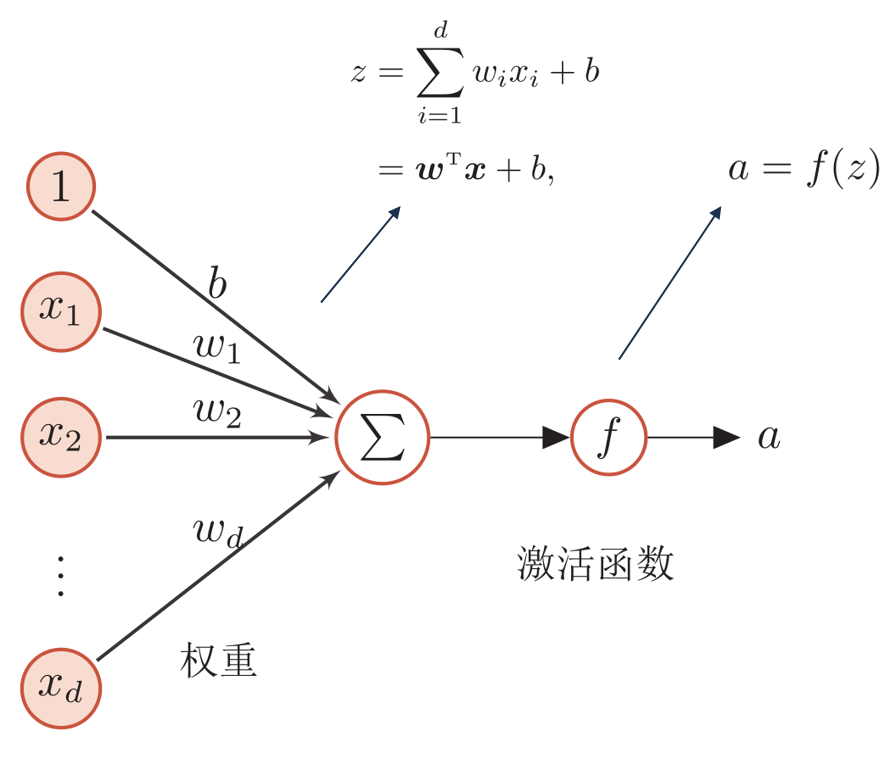
\includegraphics[width=0.6\linewidth]{人工神经元.png}
    \caption{人工神经元模型}
    \label{fig:神经元}
  \end{figure}

在图~\ref{fig:神经元}中,$\vec{x}$为输入向量,$w$和$b$分别是权重和偏移。

神经网络主要由以下几部分组成:
\begin{itemize}
    \item 输入节点(输入层)。在这一层中不进行任何计算,它们只是将信息传递给下一层(大部分时间是隐藏层)。
    \item 隐藏节点(隐藏层)。中间处理或计算在隐藏层中完成的,然后将输入层的权重(信号或信息)传递给下一层(另一个隐藏层或输出层)。一个神经网络也可以不包含隐藏层。
    \item 输出节点(输出层)。此层位于神经网络的最末层,负责接管来自前面隐藏层所输入的信息或信号。再通过激活函数,最终将得到合理范围内的理想数值,例如用于分类的softmax 函数。
    \item 连接和权重。神经元之间会有边进行连接,每条边会有一定的权重。即每个连接将神经元$i$的输出传递给神经元$j$的输入,每个连接被赋予一个权重$W_{ij}$。
    \item 激活函数。这个函数的作用在于将非线性特征引入到神经网络当中。同时它会将值的范围紧缩至更小,所以一个Sigmoid 激活函数的值区间为[0,1]。深度学习中有很多激活函数,如Sigmoid、Tanh、ReLU 、Softplus、Softmax 等。表\ref{table:激活函数}为常见的激活函数。
    \begin{table}[]
        \caption{激活函数}
        \label{table:激活函数}
        \centering
        \begin{tabular}{|l|l|l|}
        \hline
        名称&表达式&导数\\ \hline
        Sigmoid &  $f(x) = \frac{1}{1+e^{-x}}$ & $f'(x) = f(x)(1-f(x))$
        \\ \hline
        Tanh & $f(x) = \frac{2}{1+e^{-2x}} - 1$ & $f'(x) = 1 - f(x)^2$ \\ \hline
        ReLU & $f(x) = max(0, x)$ & $f'(x)=\begin{cases}
        0& \text{x<0}\\
        1& \text{x>=0}
        \end{cases}$ \\ \hline
        Softplus & $f(x) = log(1+e^x)$ & $f'(x) = \frac{e^x}{1+e^x}$ \\ \hline
        Softmax & $S_i = \frac{e_i}{\sum_j e_j}$ & \\ \hline
        \end{tabular}
        \end{table}
    \item 学习规则。利用学习规则修改神经网络中的权重和阈值。
\end{itemize}

\subsection{RNN}

下图~\ref{fig:循环神经网络}是循环神经网络的示意图\cite{rnn-structure}。
\begin{figure}
    \centering
    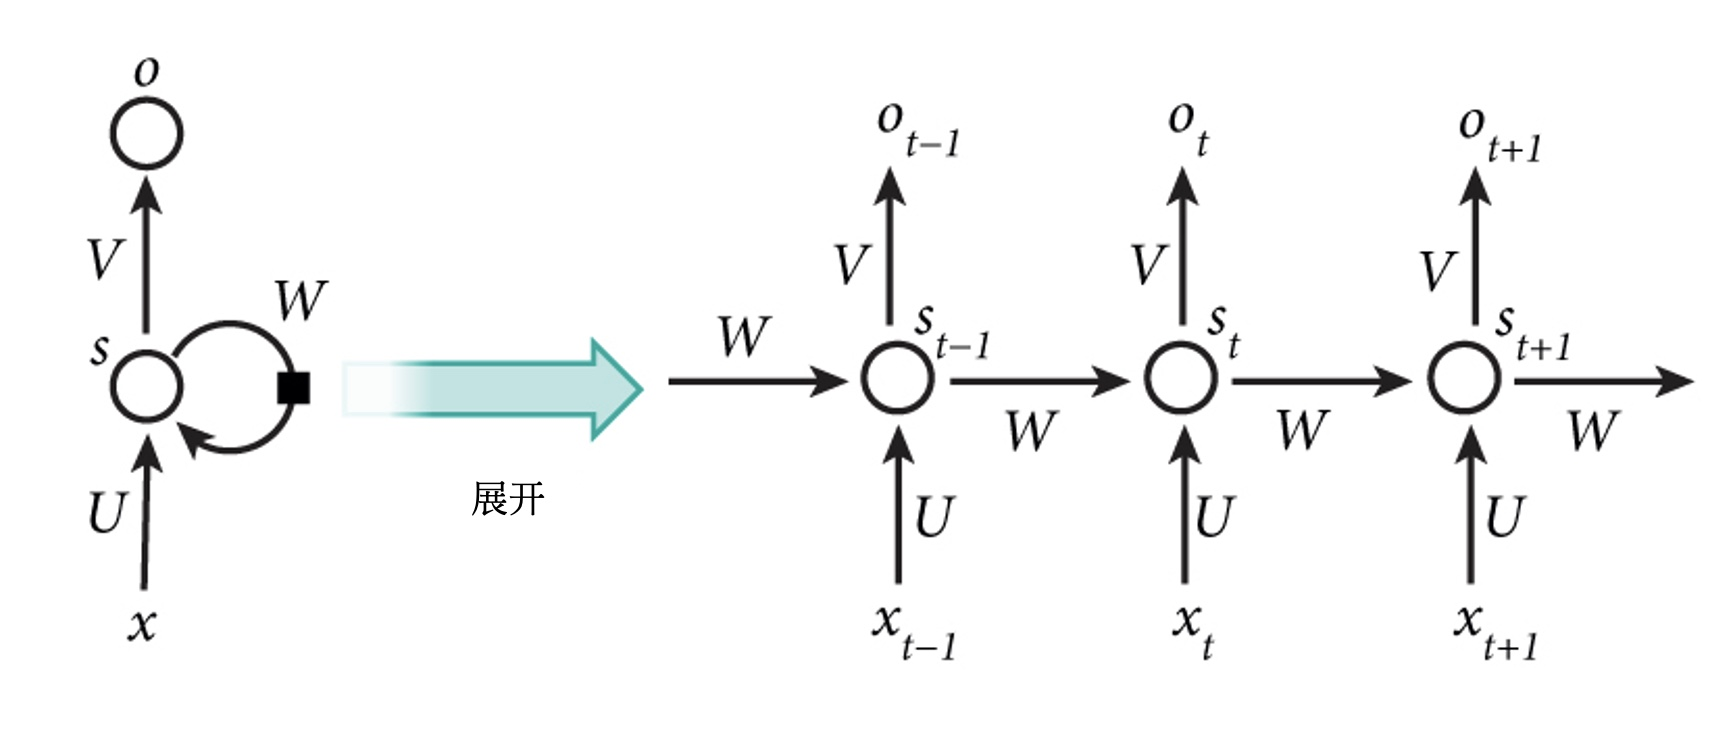
\includegraphics[width=0.6\linewidth]{循环神经网络.jpg}
    \caption{循环神经网络}
    \label{fig:循环神经网络}
  \end{figure}
该图显示了一个循环神经网络被展开成一个完整的神经网络。例如,如果输入序列是时间窗口为T的一组向量,那么网络会被展开成T层的神经网络。
  用公式表示如下:
  \begin{equation}
      \begin{aligned}
          O_t &= g(V\cdot S_t) \\
          S_t &= f(U\cdot X_t + W\cdot S_{t-1})
      \end{aligned}
  \end{equation}

  $x_t$表示第$t$步的输入,例如$x_1$表示时刻1的特征向量。$s_t$表示第t步隐藏层状态,也就是网络中的“记忆”。获得$s_t$的过程是计算位于之前的隐藏层状态及当前层的输入向量。函数$f(\cdot)$通常是一个非线性函数,如tanh或者ReLU。

RNN伪代码如算法\ref{RNN伪代码} 所示,架构图如图\ref{fig:普通RNN结构}所示\cite{rnn-structure}。
  \begin{algorithm}[!h]
    \caption{\emph{RNN伪代码}}
    \label{RNN伪代码}
    \begin{algorithmic}[1]
      \Require t时刻的特征向量
      \Ensure t+T时刻的特征向量
      \State 初始化t时刻单元状态
      \For{t $\leftarrow$ $1$ to $T$}
        \State $output_t = activation(input_t, state_t)$
        \State $state_t$ = $output_t$
      \EndFor
    \end{algorithmic}
  \end{algorithm}

\subsection{LSTM}
普通RNN有不能处理长依赖的问题,因此Hochreiter提出了一种长短期记忆网络-LSTM,LSTM是一种特殊的RNN,适用于学习长期依赖。现在LSTM已经被广泛应用于各个领域。如图\ref{fig:LSTM结构}所示\cite{rnn-structure}, LSTM和RNN类似,网络中都具有链式结构,但是LSTM中的循环单元与RNN中简单的$tanh$层不同,其构建了一些“门”(Gate)。利用构建出的“门”单元,能够将历史信息保留在当前节点状态,具体来说,是保留那些权重高的单元删除权重低的单元。
% 让神经网络记住很久之前的重要信息或者忘记最近的不重要信息。

% 所有RNN都具有链式形式。在普通的RNN中,这种循环是一种非常简单的结构,比如简单的tanh层。
\begin{figure}
    \centering
    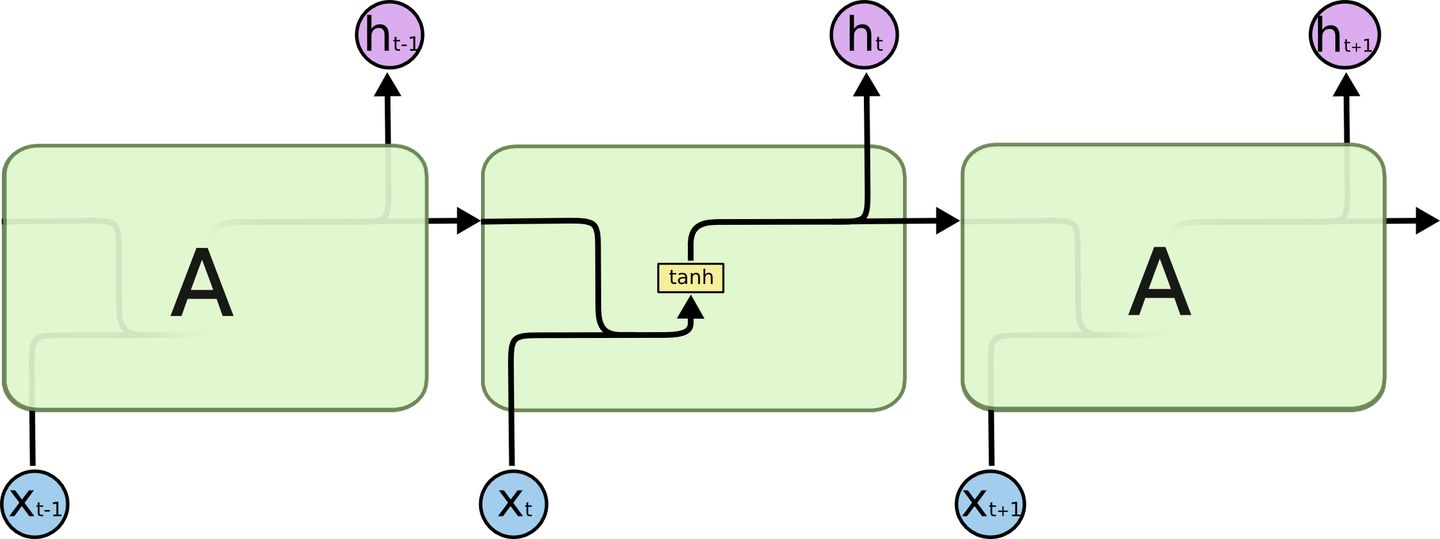
\includegraphics[width=0.6\linewidth]{普通RNN结构.jpg}
    \caption{普通RNN结构}
    \label{fig:普通RNN结构}
  \end{figure}

% LSTM也具有这种链式结构,但循环单元里面不再是只有单一的神经网络层,而是构建了一些“门”(Gate)。原来的 RNN,由于这种链式结构的限制,很长的时刻以前的输入对现在的网络影响非常小,后向传播时那些梯度也很难影响很早以前的输入,即会出现梯度消失的问题。而 LSTM 通过构建“门”,让网络能记住那些非常重要的信息,比如遗忘门,来选择性清空过去的记忆和更新较新的信息。
\begin{figure}
    \centering
    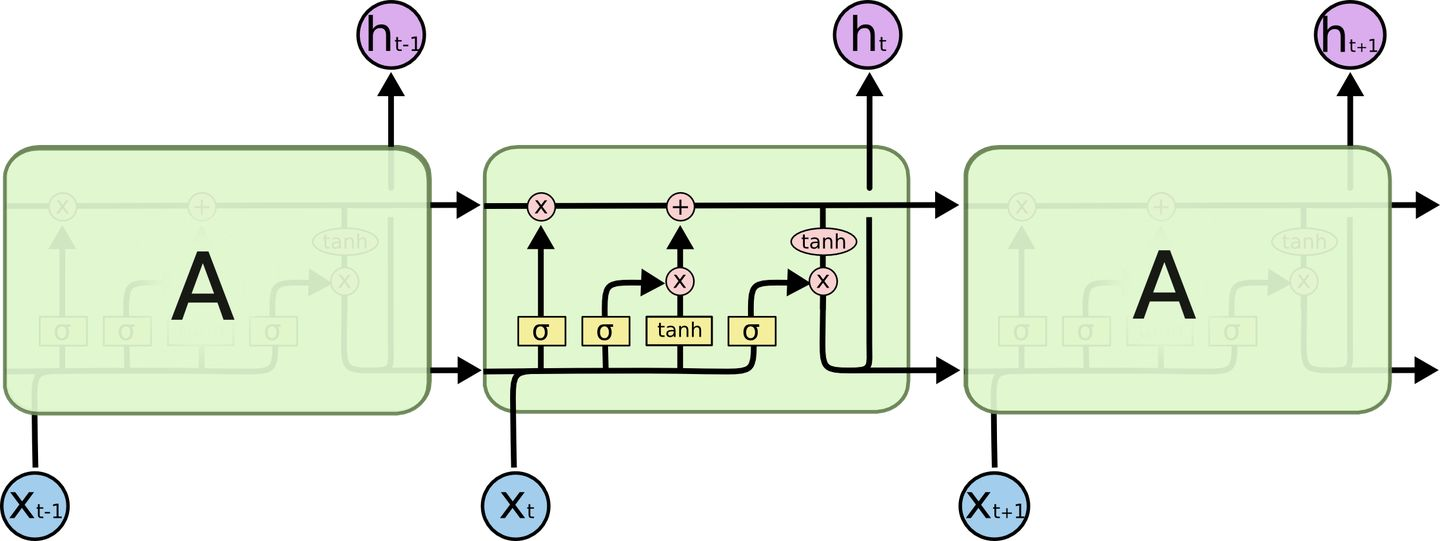
\includegraphics[width=0.6\linewidth]{LSTM结构.jpg}
    \caption{LSTM结构}
    \label{fig:LSTM结构}
  \end{figure}
  LSTM 首先通过$\sigma$层的“遗忘门”从单元状态中丢弃不重要的信息。遗忘门会读取上一时刻的输出$h_{t-1}$和当前时刻的输入$x_t$,计算出一个维度为n的向量$f_t$,该向量的值均在$[0, 1]$之间。1 表示“完全保留”上个神经元的状态信息,0 表示“完全舍弃”。

\begin{equation}
    \begin{aligned}
        f_t = \sigma(W_f\cdot x_t + U_f\cdot h_{t-1} + b_f)
    \end{aligned}
\end{equation}

下一步是确定该神经元的哪些新状态信息被存放在单元状态中。这里包含两个部分。第一,sigmoid 层,即 “输入门层” ,决定LSTM单元将更新哪些值。然后, tanh 层创建一个新的候选值$z_t$的向量,该向量可以加入到下一层单元状态中。

\begin{equation}
    \begin{aligned}
        i_t = \sigma(W_i\cdot[h_{t-1},x_t] + b_i)
    \end{aligned}
\end{equation}

\begin{equation}
    \begin{aligned}
        \widetilde {C_t} = tanh(W_C\cdot[h_{t-1},x_t]+b_C)
    \end{aligned}
\end{equation}
最后一步是将旧单元状态$c_{t-1}$更新为新状态$c_t$。把旧状态与遗忘门$f_t$相乘,丢弃掉之前无需保留的信息,接着与新状态进行相加,综合得出该神经元的输出的状态,也即更新单元的状态。
\begin{equation}
    \begin{aligned}
        C_t = f_t * C_{t-1} + i_t * \widetilde{C_t}
    \end{aligned}
\end{equation}


\begin{algorithm}[!h]
  \caption{\emph{LSTM伪代码}}
  \begin{algorithmic}[1]
      \Require 一组按时间排列的向量组
      \Ensure 按时间排列的向量组
      \State $\vec C_0 = \vec 0$
      \State $\vec h_0 = \vec 0$
      \For{$t$ \leftarrow $1$ to $T$}
      \State $output_t = activation(dot(W, input_t) + dot(U, state_t) + b)$
      \State $state_t = output_t$
      \State $i_t = activation(dot(state_t,))$
      % output_t = activation(dot(state_t, Uo) + dot(input_t, Wo) + dot(C_t, Vo) + bo)
      % #输入门
      % i_t = activation(dot(state_t, Ui) + dot(input_t, Wi) + bi)
      % 遗忘门
      % f_t = activation(dot(state_t, Uf) + dot(input_t, Wf) + bf)
      % #候选记忆单元
      % k_t = activation(dot(state_t, Uk) + dot(input_t, Wk) + bk)
      
      % c_t+1 = i_t * k_t + c_t * f_t

      \EndFor
  \end{algorithmic}
\end{algorithm}


\subsection{GRU}
门控循环单元(Gated Recurrent Unit,GRU)简化了LSTM模型,不仅合并了遗忘门和输入门,也合并了单元状态和隐藏层状态,在保证训练效果的同时大大减少了参数数量。
% 循环门单元(Gated Recurrent Unit,GRU),由 Cho, et al. (2014)提出。它组合了遗忘门和输入门到一个单独的“更新门”中。它也合并了cell state和hidden state,并且做了一些其他的改变。结果模型比标准LSTM模型更简单,
\begin{figure}
    \centering
    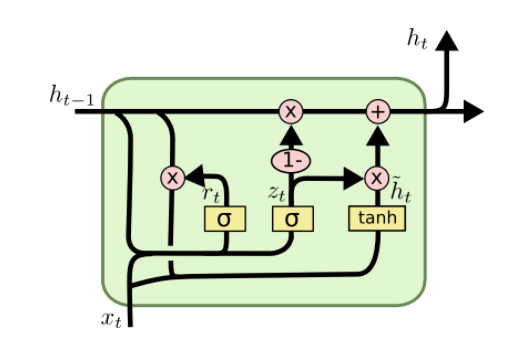
\includegraphics[width=0.6\linewidth]{GRU结构.png}
    \caption{GRU结构}
    \label{fig:GRU结构}
  \end{figure}

  \begin{equation}
    \begin{aligned}
        z_t = \sigma(W_z\cdot [h_{t-1},x_t])
    \end{aligned}
\end{equation}

\begin{equation}
    \begin{aligned}
        r_t = \sigma(W_r\cdot[h_{t-1},x_t])
    \end{aligned}
\end{equation}

\begin{equation}
    \begin{aligned}
        \widetilde {h_t} = tanh(W\cdot[r_t * h_{t-1}, x_t])
    \end{aligned}
\end{equation}

\begin{equation}
    \begin{aligned}
        h_t = (1- z_t) * h_{t-1} + z_t * \widetilde{h_t}
    \end{aligned}
\end{equation}
由图\ref{fig:GRU结构}中结构可以看出\cite{rnn-structure},GRU是通过一个循环神经网络和“门”机制来不断更新内部参数。


\section{本章小结}
本章是相关工作,首先介绍了网络流量异常的定义和分类,然后按照不同的类别综述了网络流量异常检测的常用算法,最后介绍了循环神经网络的相关原理。
